\documentclass{article}
\usepackage{graphicx}
\begin{document}
	\section*{Lsg Vorschlag ADSÜ09 A3 Maximilian Maag}
	\subsection*{Aufgabe 1}
	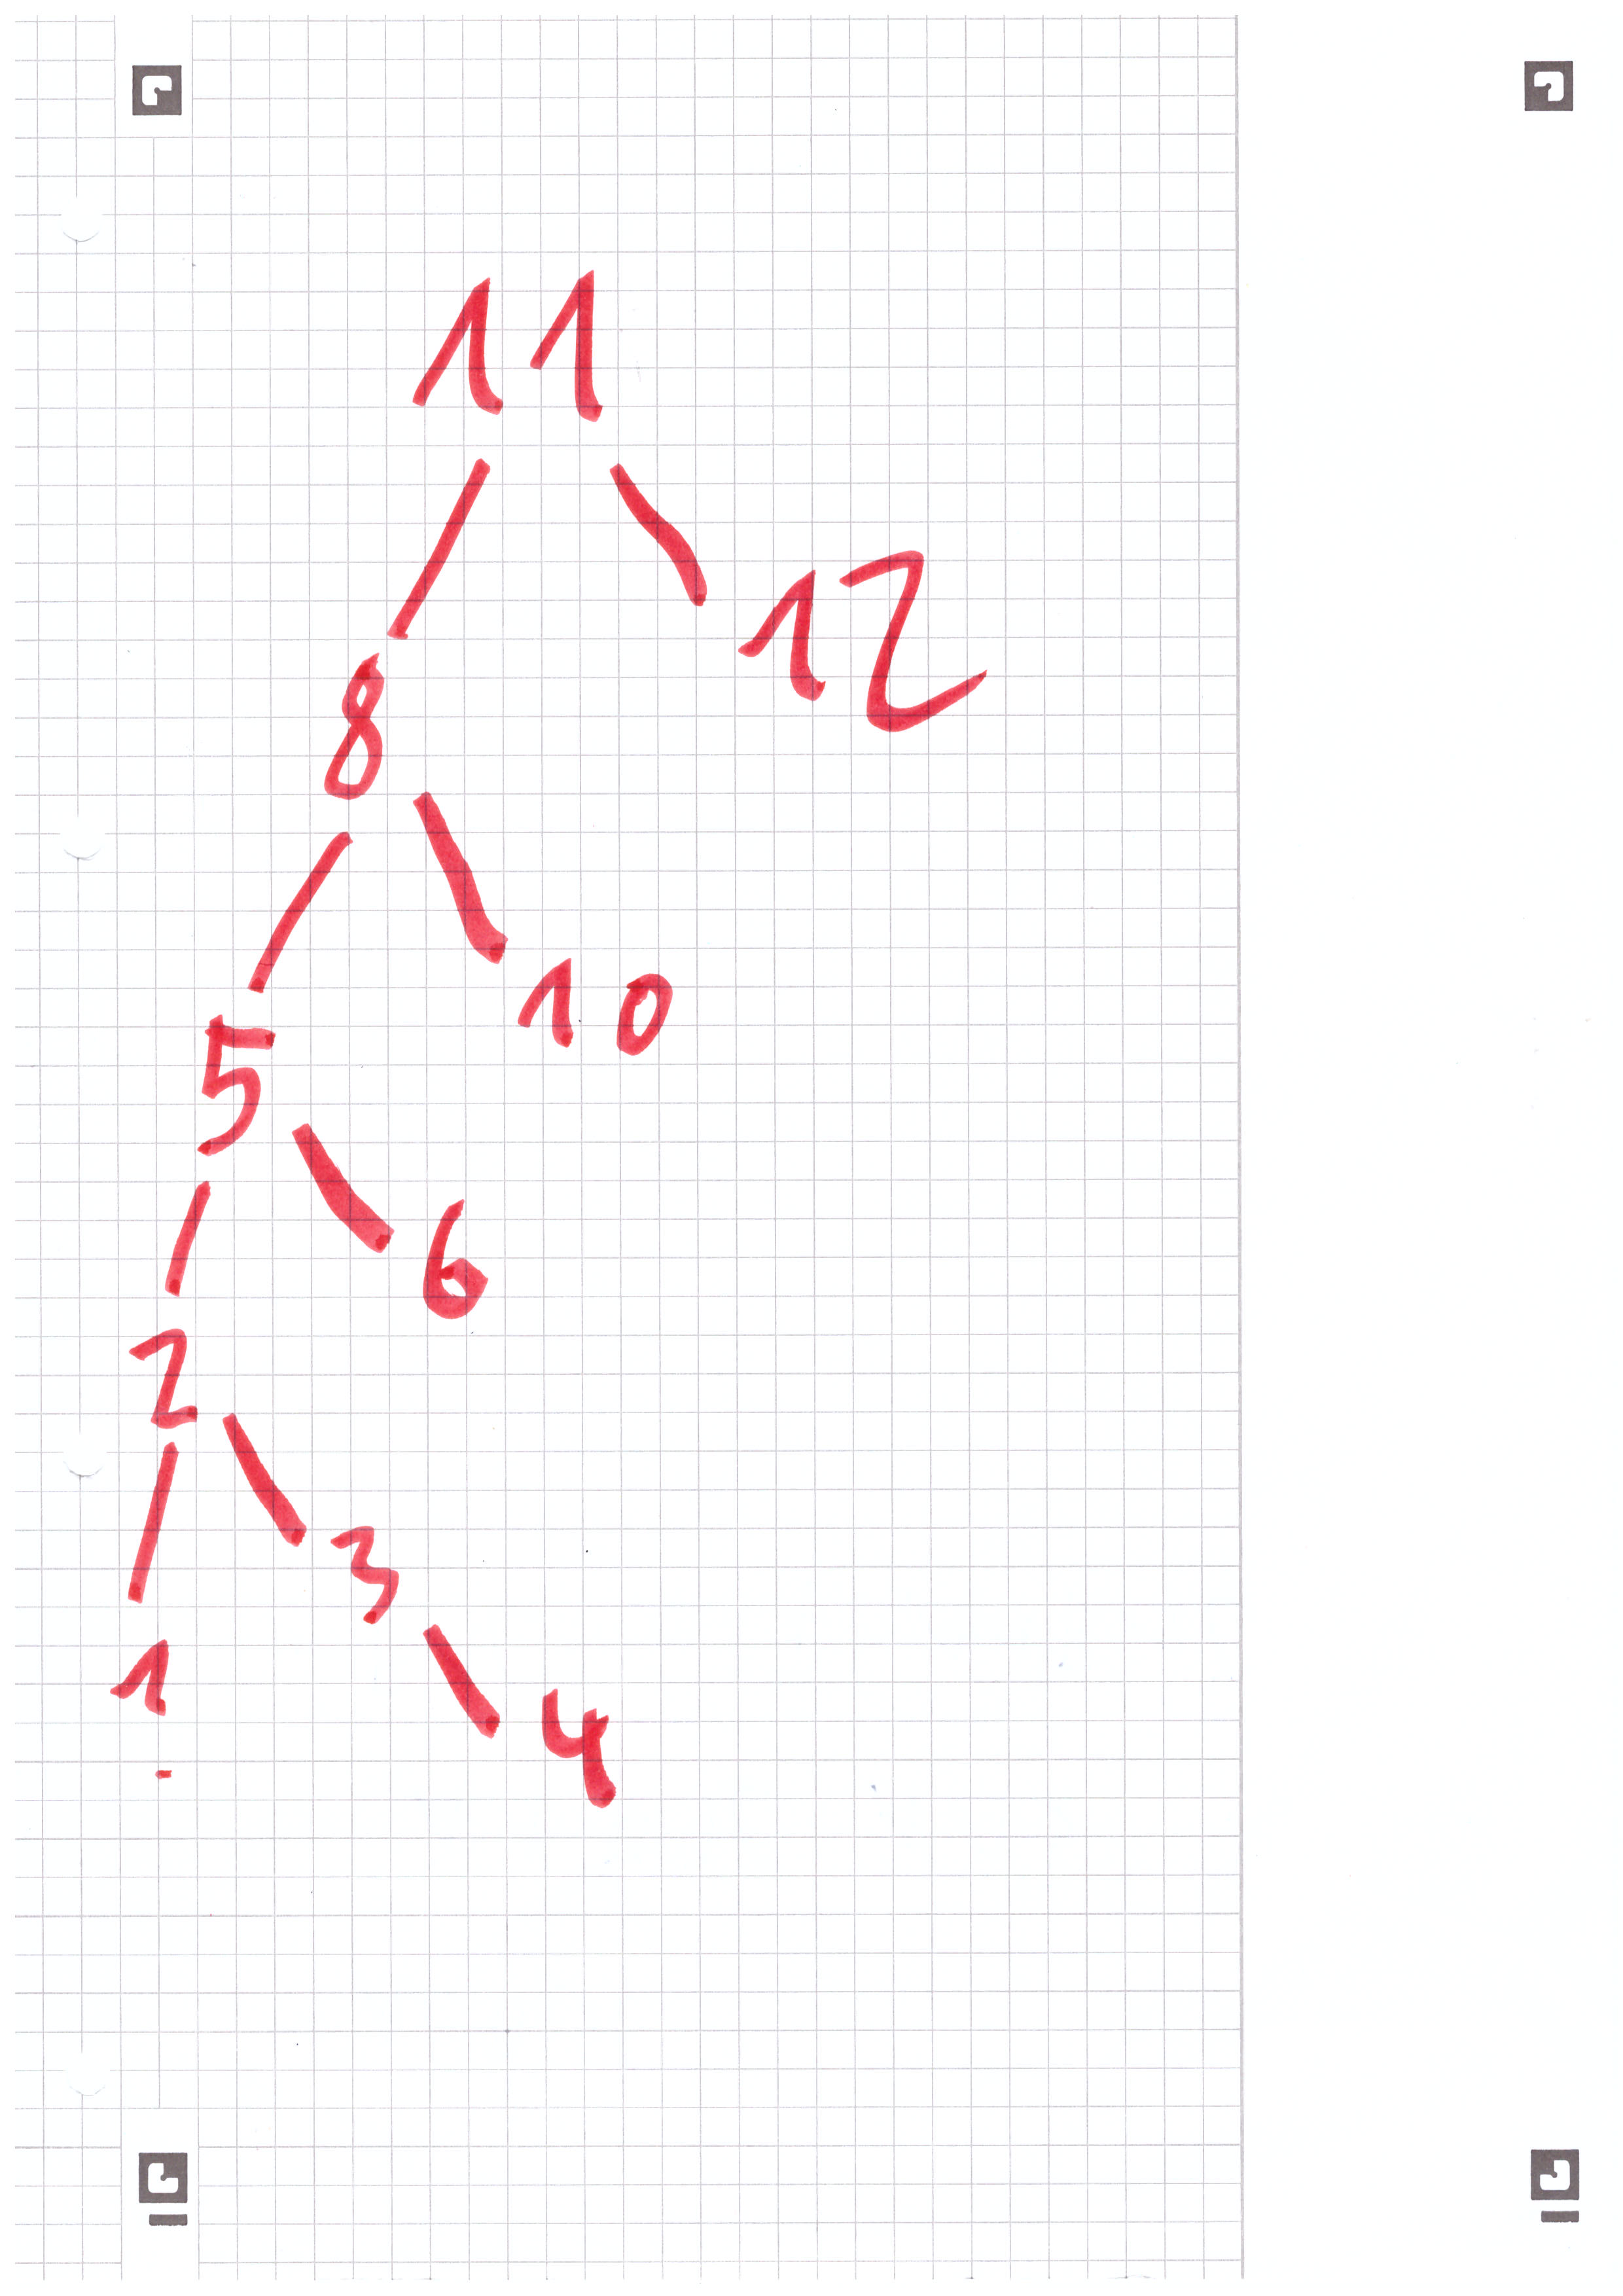
\includegraphics[width=\linewidth]{090101} \\
	SUchbaum mit entsprechenden Zahlen. \\
	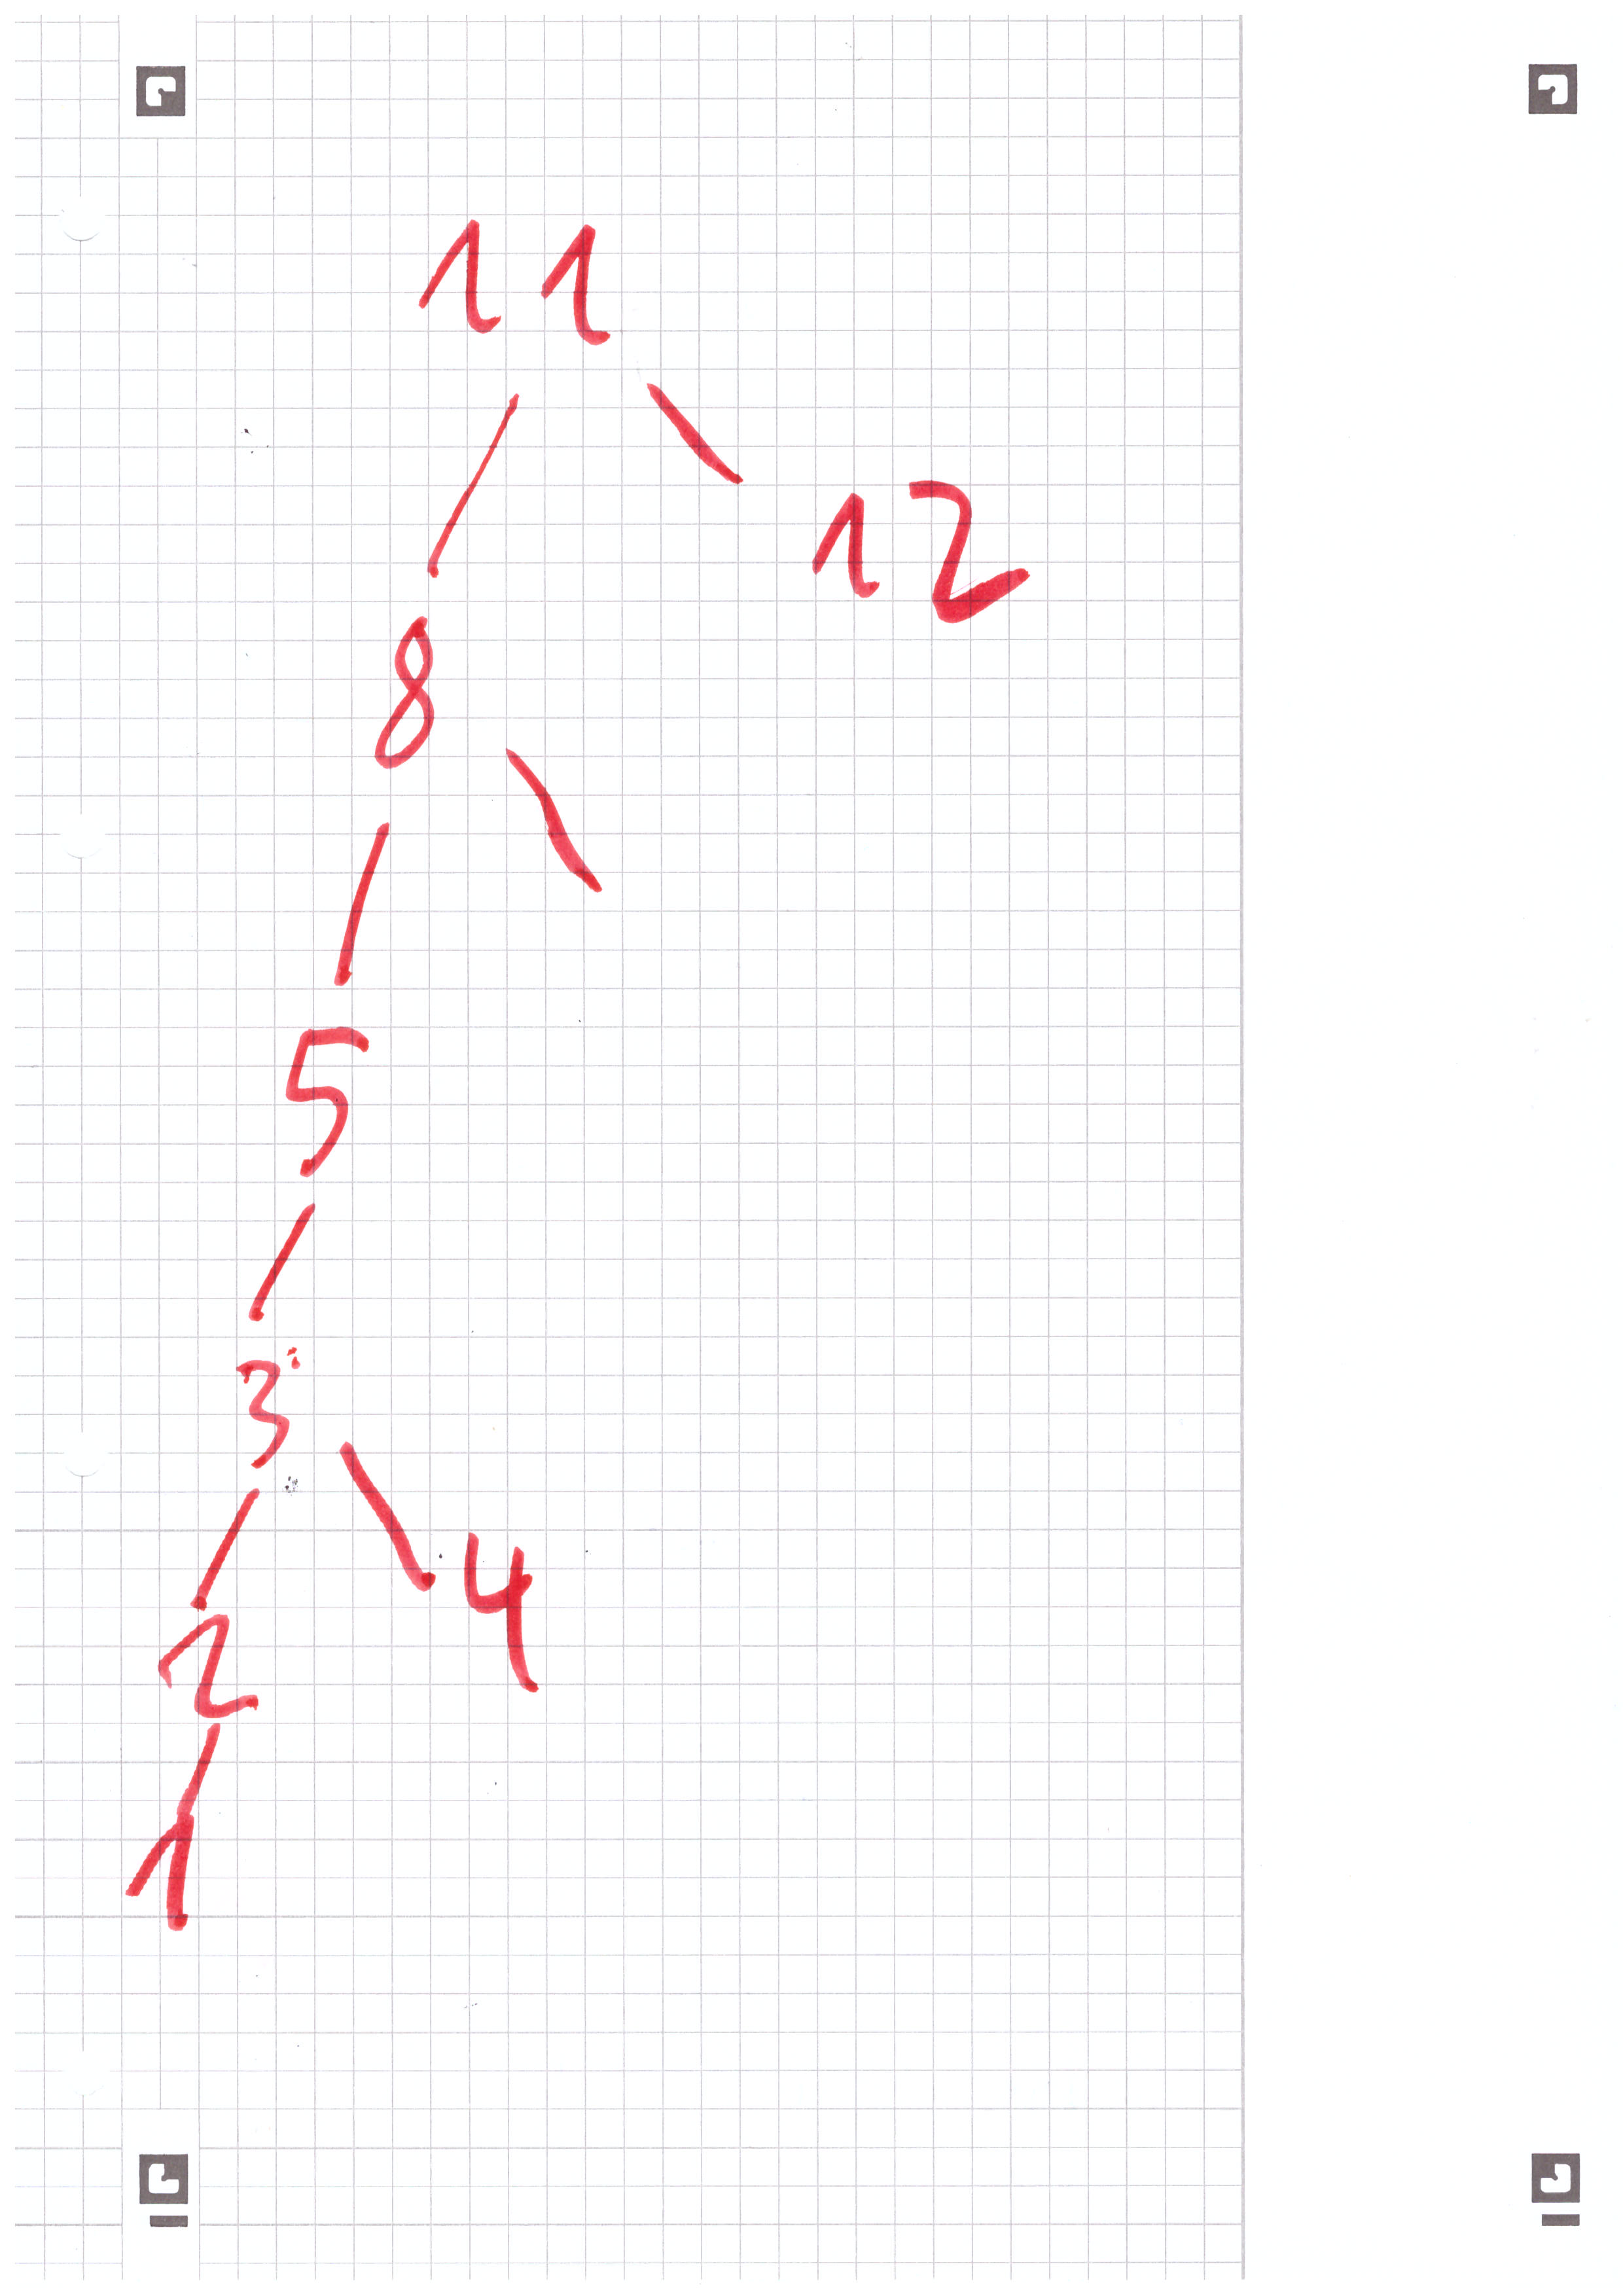
\includegraphics[width=\linewidth]{090102} \\
	Suchbaum nach der Löschung von 6 und 10.
	\subsection*{Aufgabe 2}
	Man erhält nicht immer den gleichen Suchbaum. Nachstehend ist beispielhaft illustriert wie man unterschiedliche Bäume erhalten kann. \\
	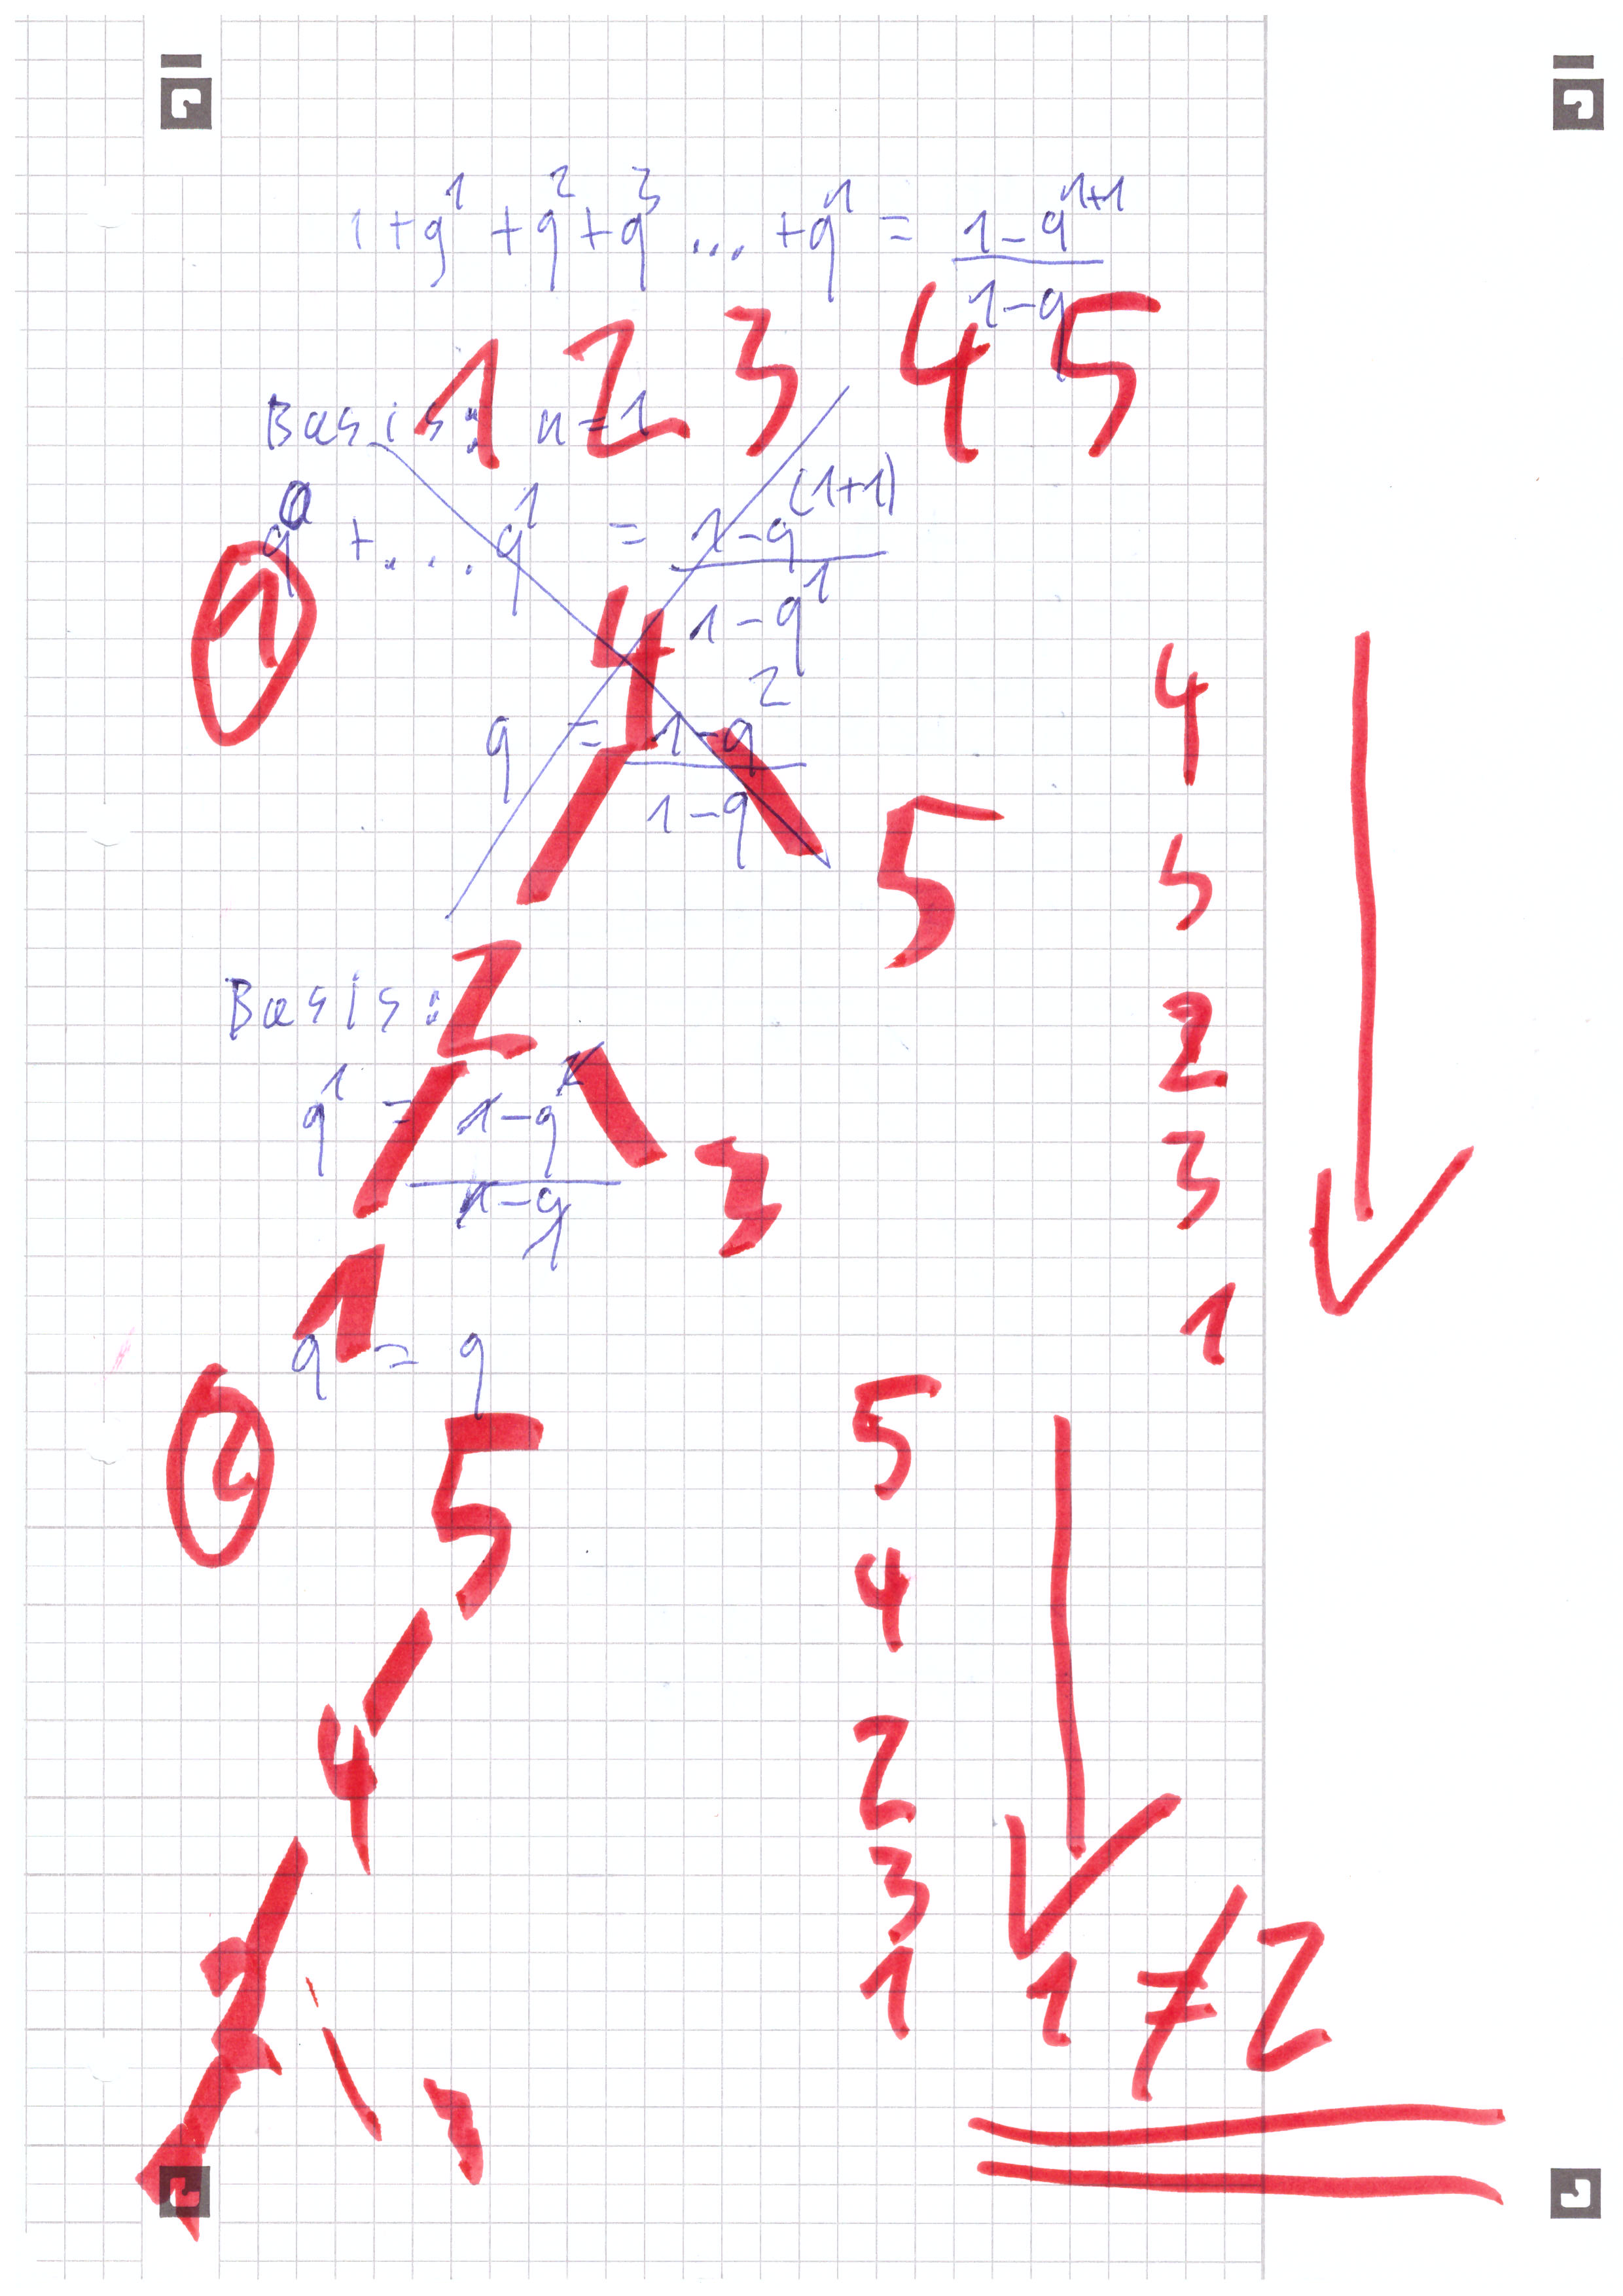
\includegraphics[width=\linewidth]{090103}
	\subsection*{Aufgabe 3}
	Best Case: \\
	Der Baum ist balanciert und besitzt die Höhe h = $log_{2}$(n).\\
	Daraus ergibt sich eine Komplexität von O(log(n)) \\ \\
	Worst Case:  \\
	Der Suchbaum ist entartet und bildet eine verkette Liste. Jedes Element der Liste muss besucht werden um dass betreffende Element zu finden und zu löschen. \\
	Daraus ergibt sich eine Komplexität von O(n).
\end{document}